\documentclass{article}\usepackage[]{graphicx}\usepackage[]{color}
% maxwidth is the original width if it is less than linewidth
% otherwise use linewidth (to make sure the graphics do not exceed the margin)
\makeatletter
\def\maxwidth{ %
  \ifdim\Gin@nat@width>\linewidth
    \linewidth
  \else
    \Gin@nat@width
  \fi
}
\makeatother

\definecolor{fgcolor}{rgb}{0.345, 0.345, 0.345}
\newcommand{\hlnum}[1]{\textcolor[rgb]{0.686,0.059,0.569}{#1}}%
\newcommand{\hlstr}[1]{\textcolor[rgb]{0.192,0.494,0.8}{#1}}%
\newcommand{\hlcom}[1]{\textcolor[rgb]{0.678,0.584,0.686}{\textit{#1}}}%
\newcommand{\hlopt}[1]{\textcolor[rgb]{0,0,0}{#1}}%
\newcommand{\hlstd}[1]{\textcolor[rgb]{0.345,0.345,0.345}{#1}}%
\newcommand{\hlkwa}[1]{\textcolor[rgb]{0.161,0.373,0.58}{\textbf{#1}}}%
\newcommand{\hlkwb}[1]{\textcolor[rgb]{0.69,0.353,0.396}{#1}}%
\newcommand{\hlkwc}[1]{\textcolor[rgb]{0.333,0.667,0.333}{#1}}%
\newcommand{\hlkwd}[1]{\textcolor[rgb]{0.737,0.353,0.396}{\textbf{#1}}}%
\let\hlipl\hlkwb

\usepackage{framed}
\makeatletter
\newenvironment{kframe}{%
 \def\at@end@of@kframe{}%
 \ifinner\ifhmode%
  \def\at@end@of@kframe{\end{minipage}}%
  \begin{minipage}{\columnwidth}%
 \fi\fi%
 \def\FrameCommand##1{\hskip\@totalleftmargin \hskip-\fboxsep
 \colorbox{shadecolor}{##1}\hskip-\fboxsep
     % There is no \\@totalrightmargin, so:
     \hskip-\linewidth \hskip-\@totalleftmargin \hskip\columnwidth}%
 \MakeFramed {\advance\hsize-\width
   \@totalleftmargin\z@ \linewidth\hsize
   \@setminipage}}%
 {\par\unskip\endMakeFramed%
 \at@end@of@kframe}
\makeatother

\definecolor{shadecolor}{rgb}{.97, .97, .97}
\definecolor{messagecolor}{rgb}{0, 0, 0}
\definecolor{warningcolor}{rgb}{1, 0, 1}
\definecolor{errorcolor}{rgb}{1, 0, 0}
\newenvironment{knitrout}{}{} % an empty environment to be redefined in TeX

\usepackage{alltt}
\usepackage{graphicx}
\usepackage{tabularx}
\usepackage{natbib}


\usepackage{array}
\usepackage{amsmath}
%\usepackage[backend=bibtex]{biblatex}
\bibliographystyle{..//refs/styles/besjournals.bst}
\setkeys{Gin}{width=0.8\textwidth}
%\setlength{\captionmargin}{30pt}
\setlength{\abovecaptionskip}{10pt}
\setlength{\belowcaptionskip}{10pt}
 \topmargin -1.5cm 
 \oddsidemargin -0.04cm 
 \evensidemargin -0.04cm 
 \textwidth 16.59cm
 \textheight 21.94cm 
 \parskip 7.2pt 
\renewcommand{\baselinestretch}{1.2} 	
\parindent 0pt

\usepackage{xr}
\usepackage{xr-hyper}
%\usepackage{hyperref}
\externaldocument{SUPPinvasive}

\title{Competition between native Honewort (\textit{Cryptotaenia canadensis}) and invasive Dame's Rocket (\textit{Hesperis matronalis}) seedlings is mediated by relative germination timing}
\IfFileExists{upquote.sty}{\usepackage{upquote}}{}
\begin{document}
\maketitle


To dos:
\begin{enumerate}
\item Update results to include niche modification question
\item Update methods to include afore mentioned models
\item
\end{enumerate}
\section*{Abstract}
\section*{Introduction}
 A central tenet of community assembly theory is that the order of arrival of species to a community mediates inter-specific interactions and can dictate the trajectory of community structure in the long term \citep{Fukami2015}. These historical contingencies, known as priority effects, have been shown to alter the structure and function of communities, driving communities to alternate stable states \citep{Fukami2011}. In many ecosystems, plant communities must re-assemble each year after a period of dormancy. In these communities, priority effects are the products of phenology, the timing of seasonal life cycle events, and the rate at which dormant plants and seeds respond to their environment and resume growth or germinate when favorable conditions return \citep{Rudolf:2019aa}.%, rather than the the timing of the arrival of propagules, which in many cases occurs prior to the dormant season \citep{Howe:1982aa,Baskin:1988aa}. 
%These seasonal, or short-term priority effects \citep{Wainwright_2011,Young:2017aa}, may be important mediators of plant interactions, and have been invoked to explain the competitive dominance of some species (when strong competitors also have rapid/early germination) \citep{Gioria2018}, and inter-specific coexistence (when weaker competitors have rapid/early germination and/or priority varies over time) \citep{Towers:2020aa}.

Invasive plants are often characterized by rapid germination and precocious phenology under a wide variety of environmental condition \citep{Gioria2018,Gioria:2017wo,Wolkovich:2011uh,Smith:2013uj}. By contrast, native plants, tend to exhibit more constrained germinations cues\citep{Marushia:2010ug}, producing seed with physiological dormancy that is released by temperature cues such as cold stratification (prolonged exposure to cool temperature) temperatures to break dormancy and stimulate germination \citep{Brink:2013wr,Cavieres:2017aa,Bradford:2007tj} .% Say better here based on Gioria

These differences in germination physiology can yield strong differences in the relative germination phenology of invasive and native plants, with invaders germination well before their native competitors (hereafter: seasonal advantage)\citep{}. This seasonal advantage can contribute significantly to the competitive abilities, and ultimately invasion success of invasive plants by allowing them to begin drawing down seasonal resources and modifying their environment before their native competitors emerge \citep{Kardol2013}. We refer to this effect of seasonal advantage on competition among species as a seasonal priority effect \\citep{Wainwright_2011,Young:2017aa}}.

Yet, it is difficult to quantify the contribution of germination seasonal priority effects to the competitive success of invaders. Germination is notorious difficult to monitor in the field, and rapid phenology often co-varies with other competitive traits % such as high fecundity, growth rates, and stress tolerance 
\citep{Dickson2012,Milbau:2003vt,HAO:2009vh} and the relative importance of seasonal advantage vs. other competitive traits to invasion success and competition dynamics in general is unknown.

Understanding the role that phenological advantage plays in mediating the dynamics
inter-specific competition is critical for predicting and managing the structure and function of plant communities in the face of anthropogenic climate change. Due  to inter-specific differences in germination response to environmental variation, the sustained alterations to environmental conditions are already shifting-community wide patterns of germination. If the patterns are indeed tightly link the the competitive dynamics of communities than phenological reorganization is likely to shift balances of species' interactions, change patterns of invasion, and strongly influence biological filtering of communities. 

\textbf{Work on this:} To address this gap, we leveraged the difference in species germination responses to the environment to quantifying how seasonal advantage among species varies with climate variation. First we performed a series of germination assays in controlled environments temperature regimes to estimate a realistic range of climate-driven variation in germination phenology between widespread invasive and native forbs. With this understanding in hand, we then performed competition trial for these species under contrasting environmental regimes to manipulate the relative germination phenology and quantify the contribution of seasonal priority effect to competitive dynamics among them.
% Compete them to assess the influences of priority effect on competitive outcome and quantify SPE's contribution vs. other intrinsic competition traits.
%Yet the differential sensitivity to the environmental cues that is driving shifts in community patterns of phenology can also be leveraged to evaluate the role of seasonal priority effect is inter-specific competition. Because germination conditions vary among years, that germination responses between competing species will converge and diverge periodically over time, depending the their specific sensitives and the climate they experience. This variation can be leverage for mechanistic tests of SPEs by quantifying how the phenological lag between species changes under realistic climate variation and the effect of this variation on competition.
%In ecological systems where dormancy release is controlled by temperature, cohabiting species respond with different sensitivities to these elements; and this is be especially true for invasive species which evolved under different climate condition in their home vs. invaded ranges \citep{}.
%\item And climate elements vary over time
%\item Together, this suggests that germination or phenological responses between competing species will converge and divirge periodically over time, depending the their specific sensitives and the climate they experience.
%\item This variation can be leverage for mechanistic tests of SPEs by a) qunatify how the phenoligical lag between species changes under realistic climate variation , and b) the effect of this variation on competition
%\section{Introduction}
%\textbf{A core task of invasion biology it to identify trait that make a species likely do be invasive}
%\begin{enumerate}
%\item Invasive species are characterized by rapid germination and precocious phenology
%\item Being so early may function as a seasonal priority effect-niche premption and such
%\item This seasonal priority effect might contribute to the competitive dominacne and invasion success of invasives
%\end{enumerate}
%\textbf{But it is difficult to infer mechanism from observational studies}
%\begin{enumerate}
%\item Because rapid phenology often covaries with other competitive traits. You'd need super high resolution phenolgy and %climate data.
%\end{enumerate}

%\textbf{Experiments can test role of SPE's in plant competition}
%\begin{enumerate}
%\item  A common approach is to use sequential planting studies.
%\item recent review paper on these experiments by \citet{Weidlich:2020aa}: 42\% of such studies included planting interval treatments of less than 1 month, approximating the time scale of SPEs and all found evidence of priority effects. (How many were invasive vs. native?)
%\end{enumerate}

%\textbf{Yet the extent to which these studies are generailizable is questionable}
%\begin{enumerate}
%\item  Almost all mechanistic tests for SPEs to date have been performed using species from temperate grasslands \citep{Weidlich:2020aa}, whose germination behavior may differ substantially from taxa in other habitats \citep{Tudela-Isanta:2018aa}.
%\item In many ecosystems, plant communities must re-assemble each year after a period of dormancy. In these communities, priority effects are largely the product of the rate at which dormant plants and seeds respond to their environment and resume growth or germinate when favorable conditions return \citep{Rudolf:2019aa}, rather than the the timing of the arrival of propagules, which in many cases occurs prior to the dormant season \citep{Howe:1982aa,Baskin:1988aa}.
%\item Therefore, sequential plantings cannot address how important SPE's are in nature because the priority effect is 100\% contigent on the choice of the treatment.
%\%end{enumerate}
%\textbf{In ecological systems where dormancy is common like temperate  and boreal forest, say a few other here, environmental conditions such as temperature (cold stratification and incubate), soil moisture, and light control the release of dormancy and germination or growth.}
%\begin{enumerate}
%\item Cohabiting species respond with different sensitivites to these elements; and this may be especially true for invasive species which evolved under different climate condition in their home vs. invaded ranges.
%\item And climate elements vary over time
%\item Together, this suggests that germination or phenological responses between competing species will converge and divirge periodically over time, depending the their specific sensitives and the climate they experience.
%\item This variation can be leverage for mechanistic tests of SPEs by a) qunatify how the phenoligical lag between species changes under realistic climate variation , and b) the effect of this variation on competition
%\end{enumerate}
%\textbf{Leveraging natural climate variation to test SPEs has major beneifits}
%\begin{enumerate}
%\item SPE's are a cornerstone of community assembly theory and modern coexistence theory, and mechansitically qunatifying their contribtion in community interactions is important
%\item Anthropogenic climatic change is altering the  environments \citep{Walck2011} and changing  germination and phenology patterns. Such sustained alterations to environmental cues have potential to disrupt SPEs, shifting balances of species' interactions, changing patterns of invasion, and strongly influence biological filtering of communities..
%\item So assessing the role of SPE's in species interactions under more realistic germination environments is timely because it can be used to improve spatio-temporal predictions of species interaction under novel climate conditions.
%\end{enumerate}%
%
%\textbf{While invasibility, competion, coexistance etc is a property of individual and community interactions, pair-wise comparisons have been a useful tool to identifying and quatify mechanisms of species interactions}
%\begin{enumerate}
%\item Why am I saying this? Probably to justify the limited taxonomic scope of my study
%\end{enumerate}
%
%\textbf{Using a combination of germination assays, competition trials and climate projections, we:}
%\begin{enumerate}
%\item Quantify gernmination behavior of varying environments to estimate a realistic range of climate driven priority between an widespread invasive and native forb species. 
%\item Compete them to assess the influences of priority effect on competitive outcome and quantify SPE's contribution vs. %other intrinsic competition traits.
%\item Use relationship between climate and germination behavior to make first-pass, quick and dirtay and rough prediction about where where interactions between these two species may shift with climate change as a proof-of-concept case study to build on in the future.
%\end{enumerate}
\section*{Methods}
\subsection{Focal species}
 Dames Rocket (\textit{Hesperis matronalis}) is a herbaceous biennial/perennial species in the \textit{Brasicaeceae} originally from Eurasia, and introduced to North America in the 19th (16th?) century \citep{}. It  can rapidly invade  meadows, forest edges and woodland, forming dense, monotypic stands and excluding native vegetation \citep{}. It is currently listed as a noxious or invasive weed is several states and provinces in the United States and Canada \citep{}. Honewort (\textit{Cryptotania canadensis}) is a herbaceous perennial in the \textit{Apiaceae} family, native to forests and woodland of North America. The  habitat overlap of these two species suggests that they may compete in nature. While their apparent niche may be similar, the two species display a substantial different germination niche, making them a suitable model for our study. \textit{C. canadensis} seeds are classified with non-deep physiological dormancy and require a substantial period of cold moist stratification to release dormancy and initiate germination. While some reports suggests that cold stratification enhances germination in \textit{H. matronalis} at low incubation temperatures \citep{} several studies have demonstrated that this fresh and after-ripened (dry-stored) seeds of \textit{H. matronalis} are capable of rapid and complete germination at a wide range of spring temperatures in the temperate zone \citep{}. The dynamics suggest that the phenological advantage among the species has potential to be strong mediated by cold stratification and incubation.  

\subsection{Germination Assays}

To investigate the relationship between environmental variation and relative germination timing between competing species, we obtained seeds of 14 spring-germinating herbaceous species common to temperate forest-edges, including our focal species  \textit{C. canadensis} and \textit{H. matronalis}, from domestic plant nurseries (see Supporting Information Tab. \ref{} for details). We performed germination assays in the growth facilities of Arnold Arboretum in Boston MA (42.3074\degree N, 71.1208\degree W). We assigned seeds to a fully crossed set of twenty experimental treatments; 10 levels of of cold stratification duration (0,14,28,35,42,49,56,63,77,91 days at 4\degree C) , two levels of incubation temperature (warm--- 25\degree C:15\degree C (day/night), cool--- 20\degree C:10\degree C (day/night)).

\noindent  Prior to applying experimental treatments we performed a ``float test" in which all seeds were placed in distilled water and unfilled seeds (floating) were removed from the experiment \citep{Baskin2014}. The remaining seeds were imbibed in distilled water for 24 hours after which we placed 20 seeds per species/ treatment combination in petri dish on moist pool filter sand. We replicated each treatment combination three times. For the cold stratification treatments, we wrapped petri dishes in aluminum foil to prevent light exposure and placed them in a growth chamber at 4\degree C. After each stratification interval, we transferred the petri dishes to their assigned incubation chamber for 25 days, moistening the germination substrate as necessary to maintain maximum saturation of the medium without flooding the seeds. We check for new germinates every 2 days, defining a seed as germinated when its radical or cotyledon tissue was visible \citep{Baskin2014}. We assessed the viability of any seeds that did not germinate in the 25 day incubation trial by performing a ``crush test" in which we applied pressure to the intact seed to evaluate its condition \citep{Baskin2014}. We excluded any seeds deemed unviable from all subsequent analyses. Due to the staggering of our stratification treatments the experiment took place between 27 August- 12 December 2018.\\

\subsubsection*{Statistical analysis}
To assess inter-specific differences in the relationship between germination rate and temperature variability, we fit a Bayesian mixed-effect accelerated failure time model (AFT) with weeks of stratification and incubation temperature as fixed effects and species as a random effect. Three species, (\textit{Carex grisea}, \textit{Impatiens capendsis} and \textit{Phlox cuspidata}), did not germinate at high enough fractions in our assays to analyze, so our final analysis consisted of 11 species.\\ 

We chose an AFT model as it allowed for us to account for viable seeds that did not germinate during our incubation window, letting us robustly compare germination timing (t50 or time to 50\% germination) even among treatments with different final germination percentages in the time of the experiment\citep{Soltani:2015aa}. One drawback of this approach is that this class of models assume that all viable seeds will eventually germinate, which we would not expect to be true in nature. For this reason, we considered any estimated t50 values greater than 60 days to indicate that seeds would not reach 50\% germination under those conditions. \\ 

In addition to our full species model described above, to obtain higher resolution estimates for the germination dynamics for our two focal species we fit an additional AFT model on a subset of data including only \textit{C. canadensis} and \text{H. matronalis}. In this model we included species as a fixed effect in addition to incubation temperature and stratification duration. 

\noindent We fit the models using the R package ``brms" \citep{Burkner2018} using a weibull distribution for the model's likelihood function. We ran the model on four chains with 4000 iterations and a 3000 iteration warm up for a total of 4000 posterior draws for each parameter using weakly informative priors. We assessed  model performance through ensuring $\hat{R}$s were between 1 and 1.01 and bulk and tail effective sample sizes were high.

\subsection{Competition Trials}
%To quantify the contribution of seasonal priorty effects to inter-specific competition dynamics, we chose two species from our germination trial \textit{Cryptotaenia canadensis} and \textit{Hesperis matronalis} for competition trials. We chose these species because the germination of \textit{C. candensis} advanced strongly with increasing cold stratification, while seeds of \textit{H. matronalis} germinated rapidly under all conditions suggesting that under low stratification treatments there would be a strong priority effect between the species that would diminish as stratification time increased. Additionally \texit{H. matronilis},originally from Eurasia, is considered an invasive species or noxious weed in many parts of North America and so evaluating the role of SPE's in this species's competitive ability has potential applied benefits for the management of this species.\\
\noindent To quantify the contribution of seasonal priorty effects to inter-specific competition dynamics of our focal species, we chose two species we performed competition trials under controlled condition in a research greenhouse at the Arnold Arboretum in October 2020-February 2021. We planted seeds into 3.5 inch square pots, employing a response surface design where we varied both the overall density of seeds and proportion of each species in each pot \citep{Inouye2001}. High and low density treatments consisted of 14 and 8 seeds total seeds respectively. Our proportion treatments (100:0\%. 25:75\%, 50:50\%, 75:25\%, 0:100\% (species A :species B)) Each density by proportion treatment was replicated six times. %This design allows us to evaluate effects of inter- and intra- specific competition and density dependence independently and in association with our experimental treatment.\\

\noindent To test the effects of temporal priority on plant growth, we randomly assigned half of the pots low (45 days) and high (72 days) cold stratification treatments at 4\degree C. We staggered the start of the treatments, so that at the conclusion of the pre-treatment, all pots were transferred to a heated greenhouse maintained at 15-25 \degree C with 14 hours of supplemental light. Germination was observed daily from 24 December- 13 January and every two days from 15 January to 1 February. The locations of each pot in the greenhouse were randomly reassigned every 3 days to minimize any blocking effects on germination or growth.

\noident After 35 days, we added 1 tsp per 1 gallon of water of Peter’s 20-10-20 liquid feed fertilizer to all pots. After 62 days, we harvested the above group biomass from all pots, dried them in a oven for 48 hours at 60\degree C, and recorded the dry weight of each species/pot using a Mettler balance.\\

\subsubsection*{Statiscal analysis}
\noindent We quantified the phenological advantage between the species by subtracting the mean germination time (MGT) of \textit{H. matronalis} from that of \textit{C. canadensis} in each pot. This allowed us to evaluate the effect phenological advantage with a regression design \citep{}, with advantage values ranging from -1.3 to 9.5 (\textit{C. candensis} mean germination time 1.3 days earlier to 9.5 days later than that of \textit{matronalis}).

For each plot, we calculated the relative growth rate difference among species using the equation below modified from \citet{Connolly2005}.

\begin{align*}

RGRD &= $ ln(\frac{Y_{Cc}}{y_{Cc}}) &- ln(\frac{Y_{Hm}}{y_{Hm}}) $
%ln({Y}\frac{y})\ %- ln(\fract{Y_{Hm}}{y_{Hm}})

\end{align*}

where $Y_{Hm}$ and $Y_{Cc}$ are the final biomass of the species at the end of the experiment and $y_{Hm}$ and $y_{Cc}$ are the inital biomass of the seeds planted at the outset of the experiment. For this calculation we obtained estimates of seed mass for our focal species from the Kew Gardens Seed Information Database \citep{}.  

We then modeled the effect of seedling density of \textit{C. canadensis}, \textit{H. matronalis} and phenological advantage time using Bayesian linear regression  using the R packages ``brms''. Using weakly informative priors, we ran this model on 4 chains, with 4000 iterations per chain and a warm up of 3000 iterations, for a total of 4,000 posterior samples per parameter. The model is written below:

\begin{align*}

RGRD &= \alpha + \beta_{1}y_{Hm} + \beta_{2}y_{Cc} + \beta_{3}MGT + \epsilon

\end{align*}

where  $\beta_{1}$ and $\beta_{2}$ are the estimated effect of changing the initial biomass of seeds of each species on the RGRD, and $\beta_{3}$ is the effect of increasing the difference in MGT between  \textit{H.matronalis} and \texti{C. canadensis}. In this formulation $\alpha$ is an un-interpretable intercept \citep{Connolly2005}.



%\subsection*{Focal species}
%\subsection*{Germination Assays}
%\subsection*{Competition Trials}
%\subsection*{Data analysis}
%\textbf{Some thoughts on Connolleys RGRD models}
%\begin{enumerate}
%\item Data at the plot level which makes large assays like the one I did tractable compared with spatially explict ones like heygi index or neighborhood
%\item Also is desinged for signle season dynamics unlike Lotke-Volterra and the usual
%\item Weakness, isn't designed for monoculture treatments( which we explictely put in out study ) since you an't have the log of zero. Maybe I overcome this by %converting 0s to 00000.1

%\end{enumerate}
\section*{Results}
\subsection*{Germination advantage}
Both stratification duration and incubation temperature significantly affected the germination phenology of the species in our study (Fig. \ref{fig:musurv}, Fig. \ref{fig:AFTall}). Stratification duration advanced the germination of all species in our study, but the strength of this relationship varied among species (Fig.\ref{fig:musurv} a. ). The germination phenology of 5 species advanced with increasing incubation temperature, while for 6 species it delayed germination (Fig.\ref{fig:musurv} b. ), suggesting that for these species, our warm incubation treatment exceeded their thermal optimum.\\

Considering our focal species, \textit{H. matronalis} reach 50\% germination in under five days for all environmental treatments, always exceeded 85\% germination regardless of environmental conditions (Fig. \ref{fig:aft}). Increasing cold stratification duration and incubation temperature only marginally only enhanced the germination rate of this species (Fig. \ref{fig:aft}). By contrast, increasing incubation temperature had a negative effect of the germination rate of \textit{C. canadensis}, suggesting that the mean 20\degree C temperatures of our warm incubation treatment are supra-optimal for the species (Fig. \ref{fig:aft}). Without sufficient cold stratification (>5 weeks for low incubation and > 7 weeks for high incubation temperatures), seeds of  \textit{C. canadensis} did not reach 50\% germination during the duration of our experiment (Fig. \ref{fig:aft},Tab. \ref{tab:germcomps}). However, under high levels of cold stratification, (>7 weeks with cool incubation) germination rates of \textit{C.canadensis} began to converge on those of \textit{H. matronialis}, and at levels of stratification greater than 10-12 weeks and low incubation temperatures, the germination rate and fraction of \textit{C.canadensis} was well matched to that of \textit{H. matronalis} (Fig. \ref{fig:aft}, Tab. \ref{tab:germcomps}).

Given the strong inter-specific differences in phenological sensitivity to stratification and incubation, our results indicate that climate strongly shapes patterns of phenological assembly, and patterns of phenological advantage can highly variable due to climate variation.

\subsection*{Germination priority effects}
In our competition trials, both competitor density and phenological priority effects had a substantial influence on the competitive interactions between \textit{C. candensis} and \textit{H. matronalis}. 
%When considering the effects of competition of per capita growth rates of each species, in the absance of phenological priority (ie both species germinate at the same time) competition coefficients for both species were less that 1 (\texit{C.candensis}=X, \textit{H. matronalis}=Y, Fig. \ref{fig:Cc}), suggesting that intra-specific competition was strong than inter-specific competition, suggesting co-existence between the species \citep{}. However, with just an increase in one day of phenolical priorty, the competition coefficient for describing the effect of \textit{H matronalis} on the per capita growth of \textit{C. canadensis} became positive  (Z, Fig. \ref{fig:Cc}) , suggesting the eventual competitive exclusion of \textit{C. candensis}.
We found increasing the density of \textit{H. matronalis} seeds shifted the community relative growth rate difference towards \textit{H. matronalis}, while increasing the density of \textit{C. candensis} seed shifted the community composition towards \textit{C. candensis}, the density effect of \textit{C. canadensis} seeds was almost three times higher than that of \textit{H. matronalis} (Fig. \ref{fig:RGRD}, Tab. \ref{tab:RGRD}). Priority effects shifted community composition strongly towards \textit{H. matronalis}, and this effect was approximately equal to the density effect of \textit{H. matronalis} (Fig. \ref{fig:RGRD}, Tab. \ref{tab:RGRD}).

\subsection*{Priority effects and germination niche modification}
We found no significant differences in the final germination fraction or mean germination time of \textit {C. canadensis} between monoculture and competition plots at both low or high levels of stratification (Fig. \ref{fig:nichemod} a,b.). When taken together our results do not provide evidence that the rapid germination of \textit{H. matronalis} modified the germination environment of \textit{C. canadensis}. 

\section*{Discussion}

\subsection*{Germination advantage as a seasonal priority effect} 
In this study, we found that climate driven differences in the germination advantage among species has strong impacts on their competitive dynamics. Our model predicts that the invasive species \textit{H. matronalis} is under the majority of species' abundance levels the competitive dominant at the seedling stage (Fig. \ref{fig:3D}). Yet at reasonably high relative abundance level, environmental conditions that reduce the phenological advantage of \textit{H. matronalis}, can facilitate the competitive success \textit{C. canadensis} by mitigating \textit{H. matronalis}'s germination priority effect (Fig. \ref{fig:3D}). We found that seasonal priority effects \textit{H. matronalis} we proportionate to its abundance influence parameter (Define this earlier in the paper) (Fig. \ref{fig:RGRD}), suggesting that precocious germination is an important mechansim for its competitive dominance, and potentially invasion success.\\

While we found priority effects impacted within-year dynamics of seedlings, our experiment was not designed to the longevity of these priority effects on the longer term, among year dynamics of our focal species. Many studies suggest that these short term priority effects many be transient, though several studies that used staggered planting methods at similar scale to the phenological lags we observed in our trials saw the influence of these initial priority effect on community composition several seasons later \citep{}.  In perennial communities, these long terms dynamics are even more difficult to assess as many perennial herbs, \textit{C. canadensis} included, rely heavily on vegetative reproduction \citep{}. Because of this, the kind of seedling to seedling competition we observed in our experiment, may be less common, and therefore less important to overall community demography than competition among vegetative ramets, or between ramets and seeds \citep{}. Understanding how phenological differences across life stages of of long-lived perennial plants affects within season inter-specific competition and 

Additionally, in our experiment, there was no cost to germianting too early. it is generally accepted that optimum germination phenology is driven by a tradeoff between maximizing the growing season and the risk of exposure to damaging environmental episodes when germinating too early \citep{}. In dry grassland ecosystem, it has been demonstrated that the precocious germination of invasive has a substantial cost in water availability is too low \citep{}. In temperate forest ecosystems, the primary risk of early phenology is damage from late season frost \citep{}. Future work could further clarify the contribution of seasonal priority effects to forest community interactions by experimentally manipulating this trade-off as well.

Given these caveats, we cannot assert our study could accurately predict the long term outcomes of competition in plant communities, even between our focal species. However, our findings are likely to be most critical use conditions where seedling competition may be most important, including colonizing new habitats through range shifts, recovering from large scale disturbances, and perhaps most importantly ecological restorations.

\subsection*{Environmental drivers of seasonal priority effect}
Our results join a growing body of experiments demonstrating that relative germination phenology can function as a seasonal or short term priority effect, enhancing the performance of the earliest germinating species at the expense of later germinants \citep{}. While this effect has been primarily commonly demonstrated in experiments in which the planting of competing seeds is staggered at increasing intervals \citep{}, we were able to generate substantial variation in relative germination timing among our competing species though by opporationalizing their differential sensitivity to environmental cues.

While we observed similar effects of stratification duration on germination phenology for \textit{H. matronalis} between our germination assays and competition trials, the effect of cold stratification on the germination phenology of \textit{C. canadensis} was distinctly less pronounced in the germination trials(approximately 20 day advance in germination assays between 6 and 10 weeks of stratification Fig. \ref{fig:aft} a) vs.  approximately 4 day advance at the same stratification difference  in in the germination trials Fig. \ref{fig:nichemods}). There are several differences among these experiments that may explain these differences.

\begin{enumerate}
\item MGT vs. T50
\item Greenhouse temperatures
\item Medium
\end{enumerate}
\subsection{Seasonal priority effects and climate change}






Our results join a growing body of experiments demonstrating that relative germination phenology can function as a seasonal or short term priority effect, enhancing the performance of the earliest germinating species at the expense of later germinants \citep{}. While this effect has been primarily commonly demonstrated in experiments in which the planting of competing seeds is staggered at increasing intervals \citep{}, we were able to generate substantial variation in relative germination timing among our competing species though by opporationalizing their differential sensitivity to environmental cues. 

While experiments have done this before a major uncertainty has been the fact the germination phenology is depends on the abiotic environment. We show how the germination advantage shifts in association with changes in the abiotic envrioment. This is useful for cliamte change.

\subsection{Germination Priority Effects and Climate Change}

This link between environmental conditions, relative germination phenology and competitive dynamics suggest that shifts in environment due to anthropogenic climate change has potentially to strongly alter early stage competition among species with deeper dormancy like \textit{C. candensis} and consistent rapid germinating species like \textit{H. matronalis}. Because stratification conditions occur at intermiately low temperature ( usally 0-10  \degreeC \citep{}), global warming is likely to increase the extent of stratification conditions in some locations, while decreasing it in others \citep{}. In regions with decreasing stratification, the rapid phenology of many invasives may allow them to exploit an unoccupied phenological niche, exerting stronger seasonal priority effects on the native community and increasign the relative abundance. By contrast, in regions where stratification conditions are being maintained or increasing, native communities may be more likely to fill the early season phenological niche, more effectively resisting invasion from species with rapid germination phenology.

This bears out for our focal species but in communities as large (Fig. \ref{fig:comm}, Fig. \ref{fig:AFTall})

\subsection*{Considering the impacts of seasonal priority effects in forest communities}
While most studies on seasonal priority effects focus on grassland environments with annual taxa \citep{} we explicitly conducted our experiment with forest perennials to better understand the generality of these effects to other ecological systems. 



There has been an increasing call to increase phenological diversity in restoration planning \citep{Hess:2019vn}. Studies in  have found that including early active species in plantings can suppress the abundance of invaders in both grassland \citep{Cleland:2013wo} and forest ecosystems \citep{Schuster:2020ww}. At the same time, restoration mixes tend to lack species which fill the early season phenological niche \citep{Havens:2016vo}. The results of our study suggestion the minimizing the priority effect advantage conferred to invasive species to due rapid germination and early phenology by including species with similar, early phenological traits, could be a powerful too for managing plant invasions and restoring native ecosystems.


Things to note: Germination was poorer in competition. Medium matters. Green house temperatures were perhaps too high.
More about cliamte change implicatins

%\subsection*{From germination requirements to germnation responses}
%Both predicting germination dynamics as a response to climate change and design phenological diverse ecological restoration communities will require a conceptual shift in how germination is studied and reported. Centuries of research of seed germination has greatly advanced our understanding of the ecology and evolution of different classes of seed dormancy and the environmental requirements that allow for dormancy break and ultimately germination \citep{}. This fundamental research is generally well integrated into applied field like plant propagation and nursery production \citep{}. Today it is almost universal for native plant growers to collect and provide information on the conditions needed to facilitate dormancy break and successful germination \citep{}. The guidance is often present as threshold treatment. For example, the \textit{C. canadensis} seeds used on our experiment reportedly had a 60 day cold stratification requirement \citep{}. Our study demonstrates that ecologically important dynamics are happening both above and below this threshold.Instead of focusing on estimating threshholds, designing research experiments to characterize the dynamics of dormancy release and germination for a wide variety of species over varying climate conditions is a critical shift from improve our ability to predict demography with climate change. A variety of statistical tools now exist to do this.

%Of course, in addition to cliamte germination by with species genetic variation and gene x environment interactions like transgenerational plasticity \citep{} 

%\textbf{So many caveats:}
%\begin{enumerate}
%\item These species are perennials, seeds banks. Given our expermental constrait couldn't account for these dynamics. ie competition my happen between raments and seeds. Our simplifed experimental design doesn't address these important factors, however they add an important piece to the puzzle. 
%\item Given above, our results may be most relevant in colonization dynamics, especially in super disturbed systems where seed ins important.
%\item Limitations of RGRD models from paper
%\item We know invasives invade communities not population, two species studies are limited to predict the invasion dynamics of a species in real time
%\item What we did do was quantify the contribution of priority effect to invasion success. It's high. This suggest restorations could benefit from consider phenological diversity 
%\end{enumerate}
\bibliography{..///refs/germination.bib}
\section*{Figures}
\begin{figure}[h!]
    \centering
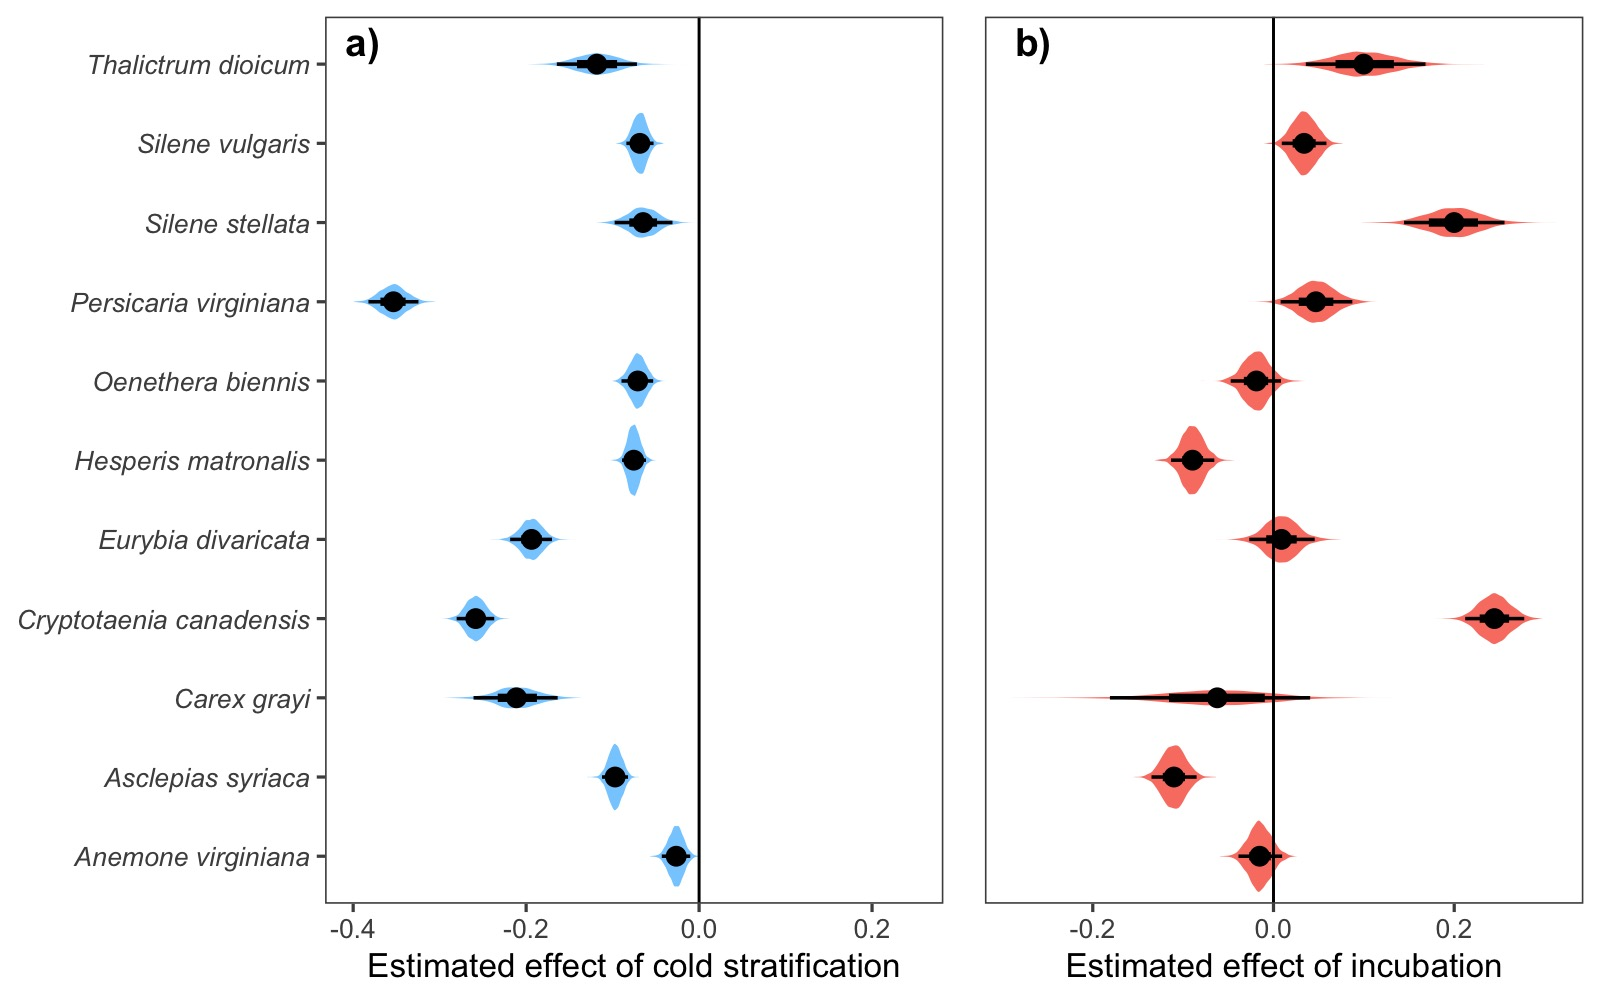
\includegraphics[width=\textwidth]{..//figure/mus_survival.jpeg}
   \caption{Estimated effects of weeks of cold stratification (\texitbf{a)}) and incubation temperature (\texitbf{b)} on the time to 50\% germination (T50) for a suite of temperate herbacious species. Negative estimates descibe an advance in T50 and positive values a delay, estimates are on the log scale. The points indicate the mean estimated effect of each parameter, thicker  and thinner bars the 50\% and 95\% credible intervals respectively. The full posterior distribution for each parameter is also dipicted  } 
   \label{fig:musurv}
\end{figure}


\begin{figure}[h!]
    \centering
         %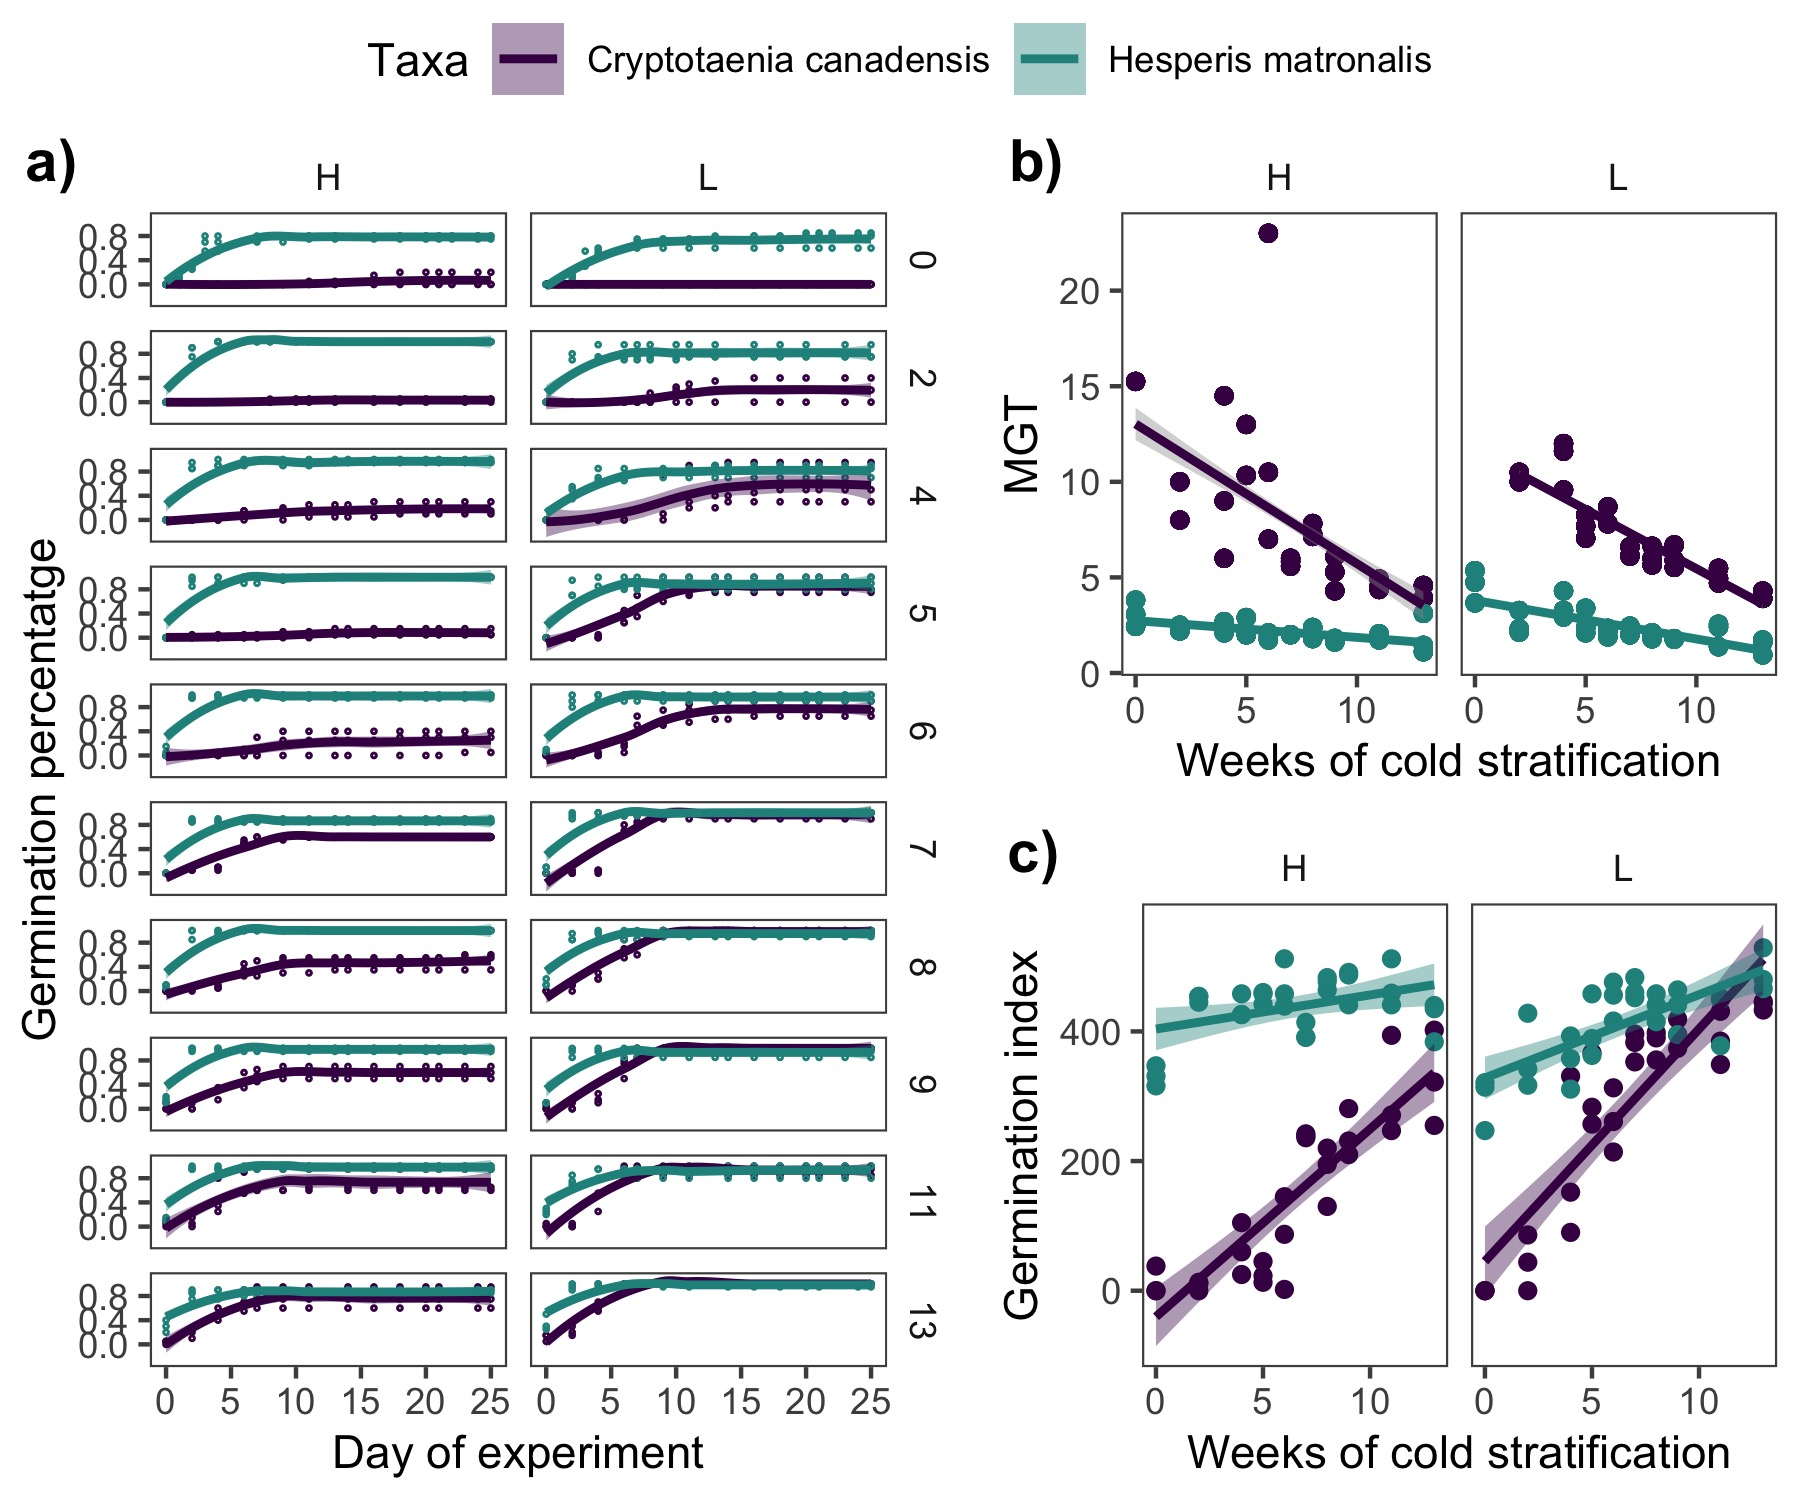
\includegraphics[width=\textwidth]{..//figure/crp_hesp1.jpeg}
          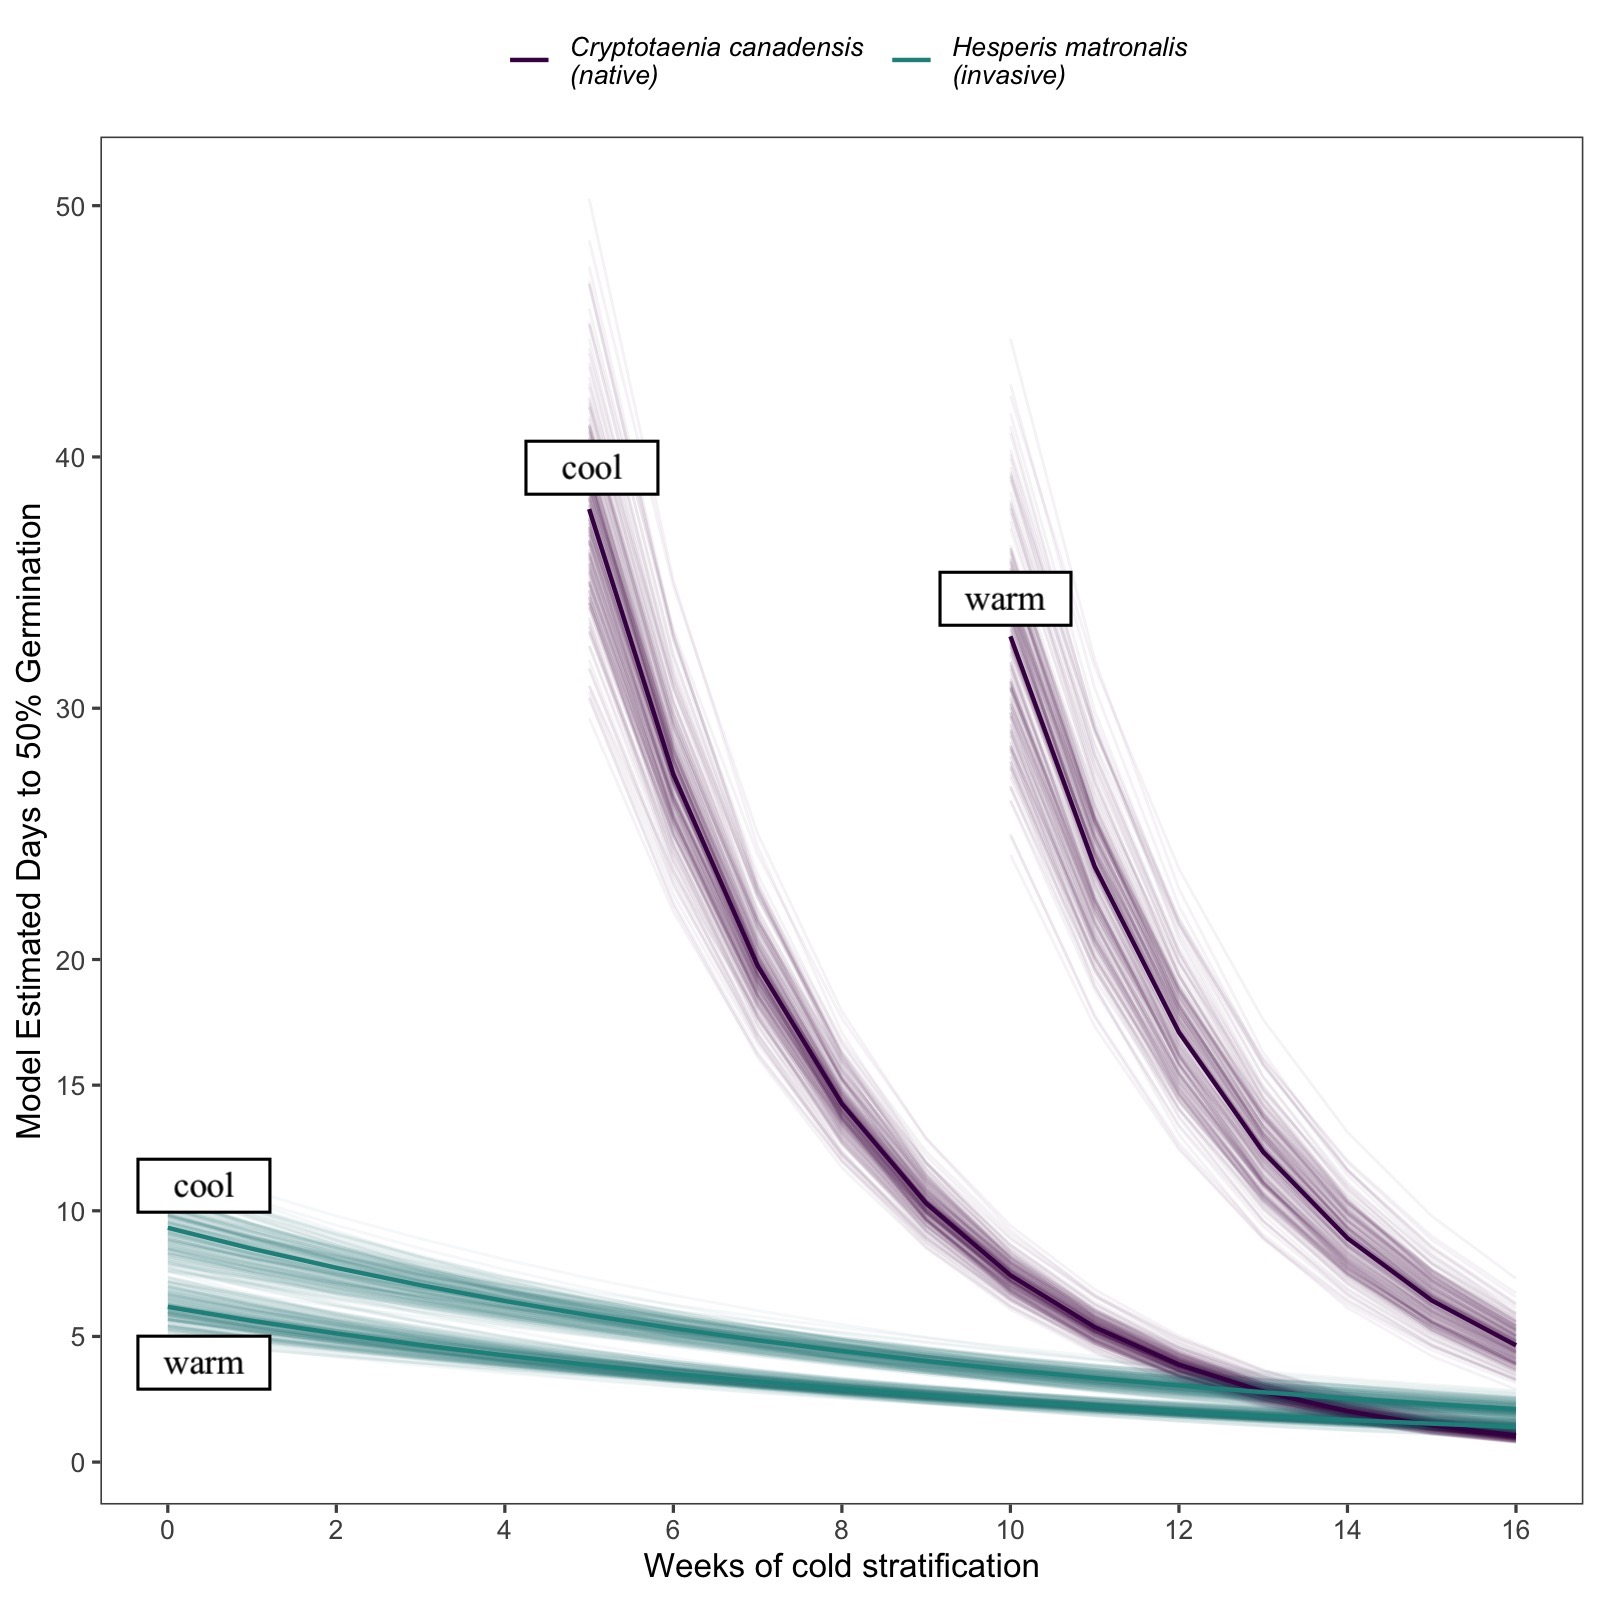
\includegraphics[width=\textwidth]{..//figure/AFTsivansive.jpeg}
%    \caption{Germination behavior of \textit{H. matronalis} and \texit{C. canadensis} indicate that the rate of \texit{C. canadensis} approaches that of \textit{H. matronalis} under cool temperatures and high levels of stratification. a) Shows germination time courses for both species at each level of incubation (H,L) and stratitification (0-13, y-axis). b) Dipicts Mean germination time for each species as a function of weeks of stratifcation and both high (H) and low (L) incubation temperature. c) Show a composite germination index for each species that account for the speed and percentage of germination for each species as a function of weeks of stratifcation and both high (H) and low (L) incubation temperature. } 
\caption{The effects of weeks of cold stratification at 4\degree C on the time to 50\% germination of \textit {Cryptotaenia canadensis} and \textit{Hesperis matronalis} under a) cool and b) warm (20/10\degree C vs. 25/15\degree C day/night) incubation conditions, estimated with accelerated failure time model. Only stratification treatment levels which allowed both species to reach 50\% germination in less that 50 days are depicted here. The solid lines indicated indicated the mean estimate, while lighter line depict uncertainly with 100 random draws from the posterior distribution.}
    \label{fig:aft}
\end{figure}


\begin{figure}[h!]
    \centering
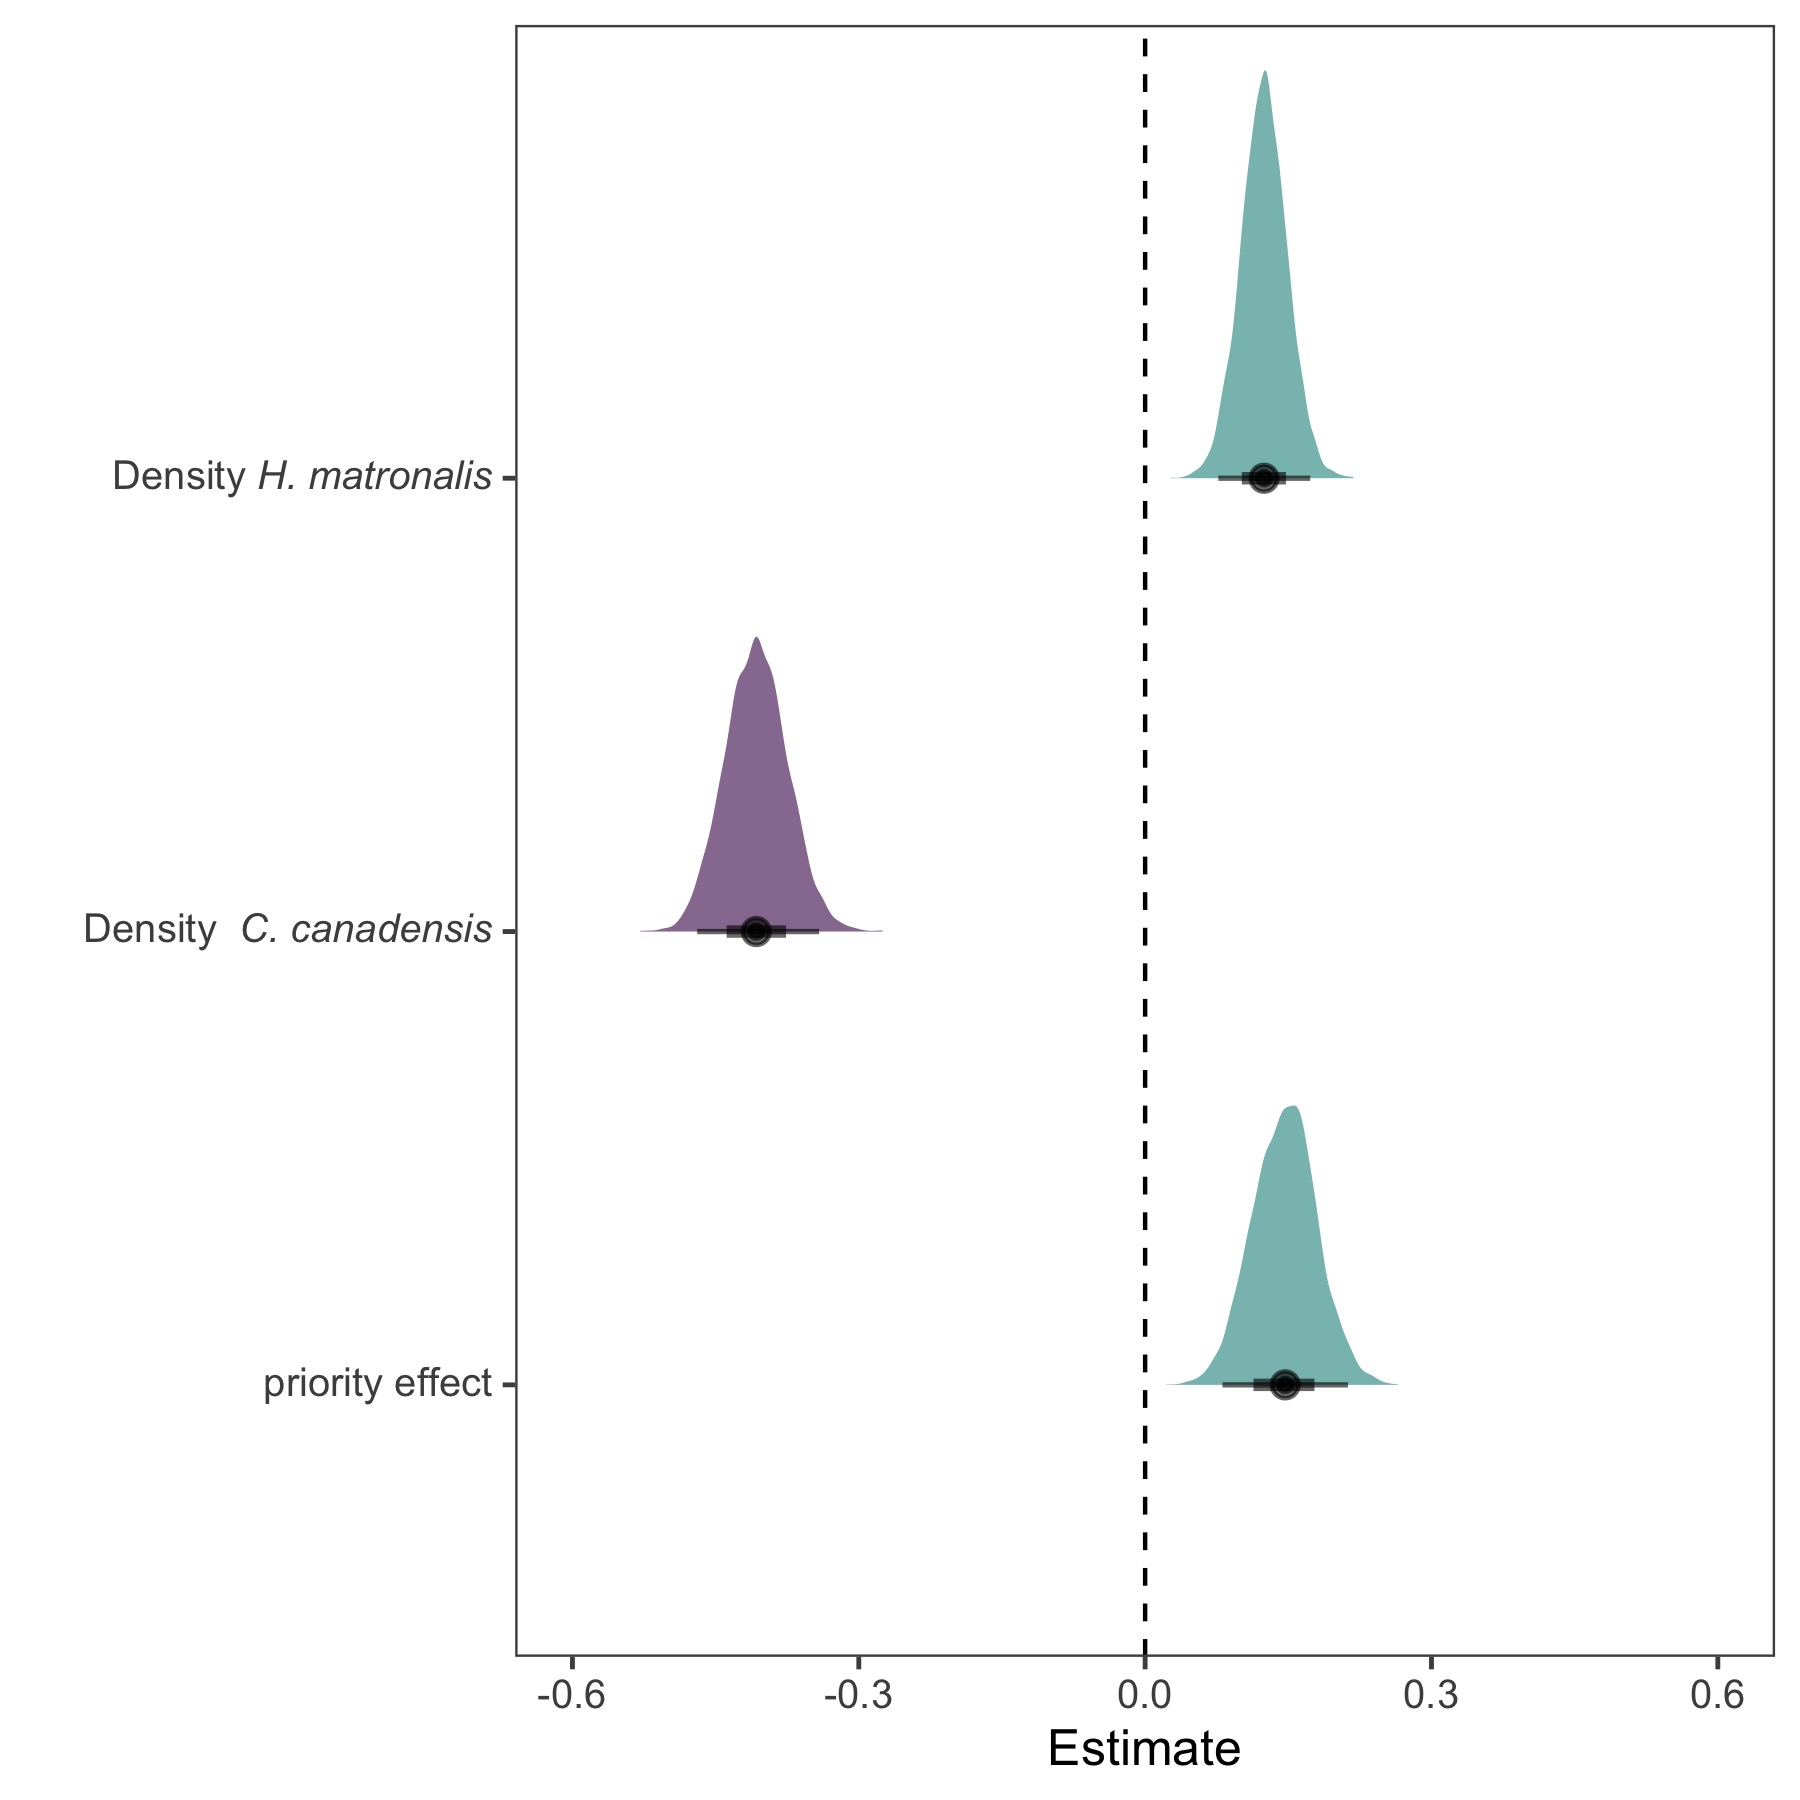
\includegraphics[width=\textwidth]{..//figure/mu_plots.jpeg}
    \caption{Estimated effects of species' abundance and phenological advantage on the relative growth rate difference between \textit{H. matronalis} and \textit{C. canadensis}. Negative parameter estimates indicate the community biomass composition shifts to favor \textit{C. candensis} while positive estimate towards dominance by \textit{ H. matronalis}. The points indicate the mean estimated effect of each parameter, thicker  and thinner bars the 50\% and 95\% credible intervals respectively. The full posterior distribution for each parameter is also dipicted. 
    } 
    \label{fig:RGRD}
\end{figure}

\begin{figure}[h!]
    \centering
\includegraphics[width=\textwidth]{..//figure/3dconnolly2.png}
   \caption{Predicted outcome of competition under differing combinations of \textit{C. canadensis} and \textit{H. matronalis} abundance and phenological advantage of \textit{H. matronalis}. Purple dots indicate conditions that favor  \texit{C. canadensis} in community biomass composition while green dot conditions favor \textit{H. matronalis}. Estimates are based on multiple regression models estimating the effect of each variable on the relative growth rate difference amoung species.} 
   \label{fig:3D}
\end{figure}

\begin{figure}[h!]
    \centering
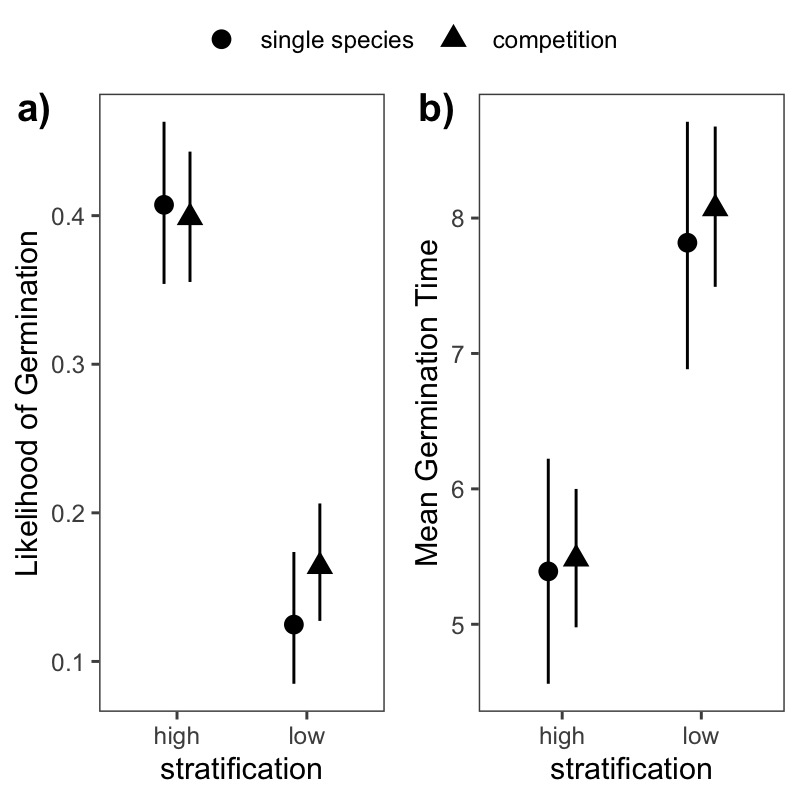
\includegraphics[width=\textwidth]{..//figure/nichemodfication.jpeg}
   \caption{Estimated effects of intra-vs. inter-specific competion on the germination dynamics of \textit{Cryptotania canadensis} under 6 (low) and 10 weeks (high) of cold stratification at 4\degree C. Panel \textbf{a)} depicts differences germination likelihood and \textbf{b)} shows the estimated mean germination time in single species mono-cultures vs. competition plot. Colored dots represent the mean estimate under each planting type and bars represent 80\% credible intervals. } 
   \label{fig:nichemod}
\end{figure}

\begin{figure}[h!]
    \centering
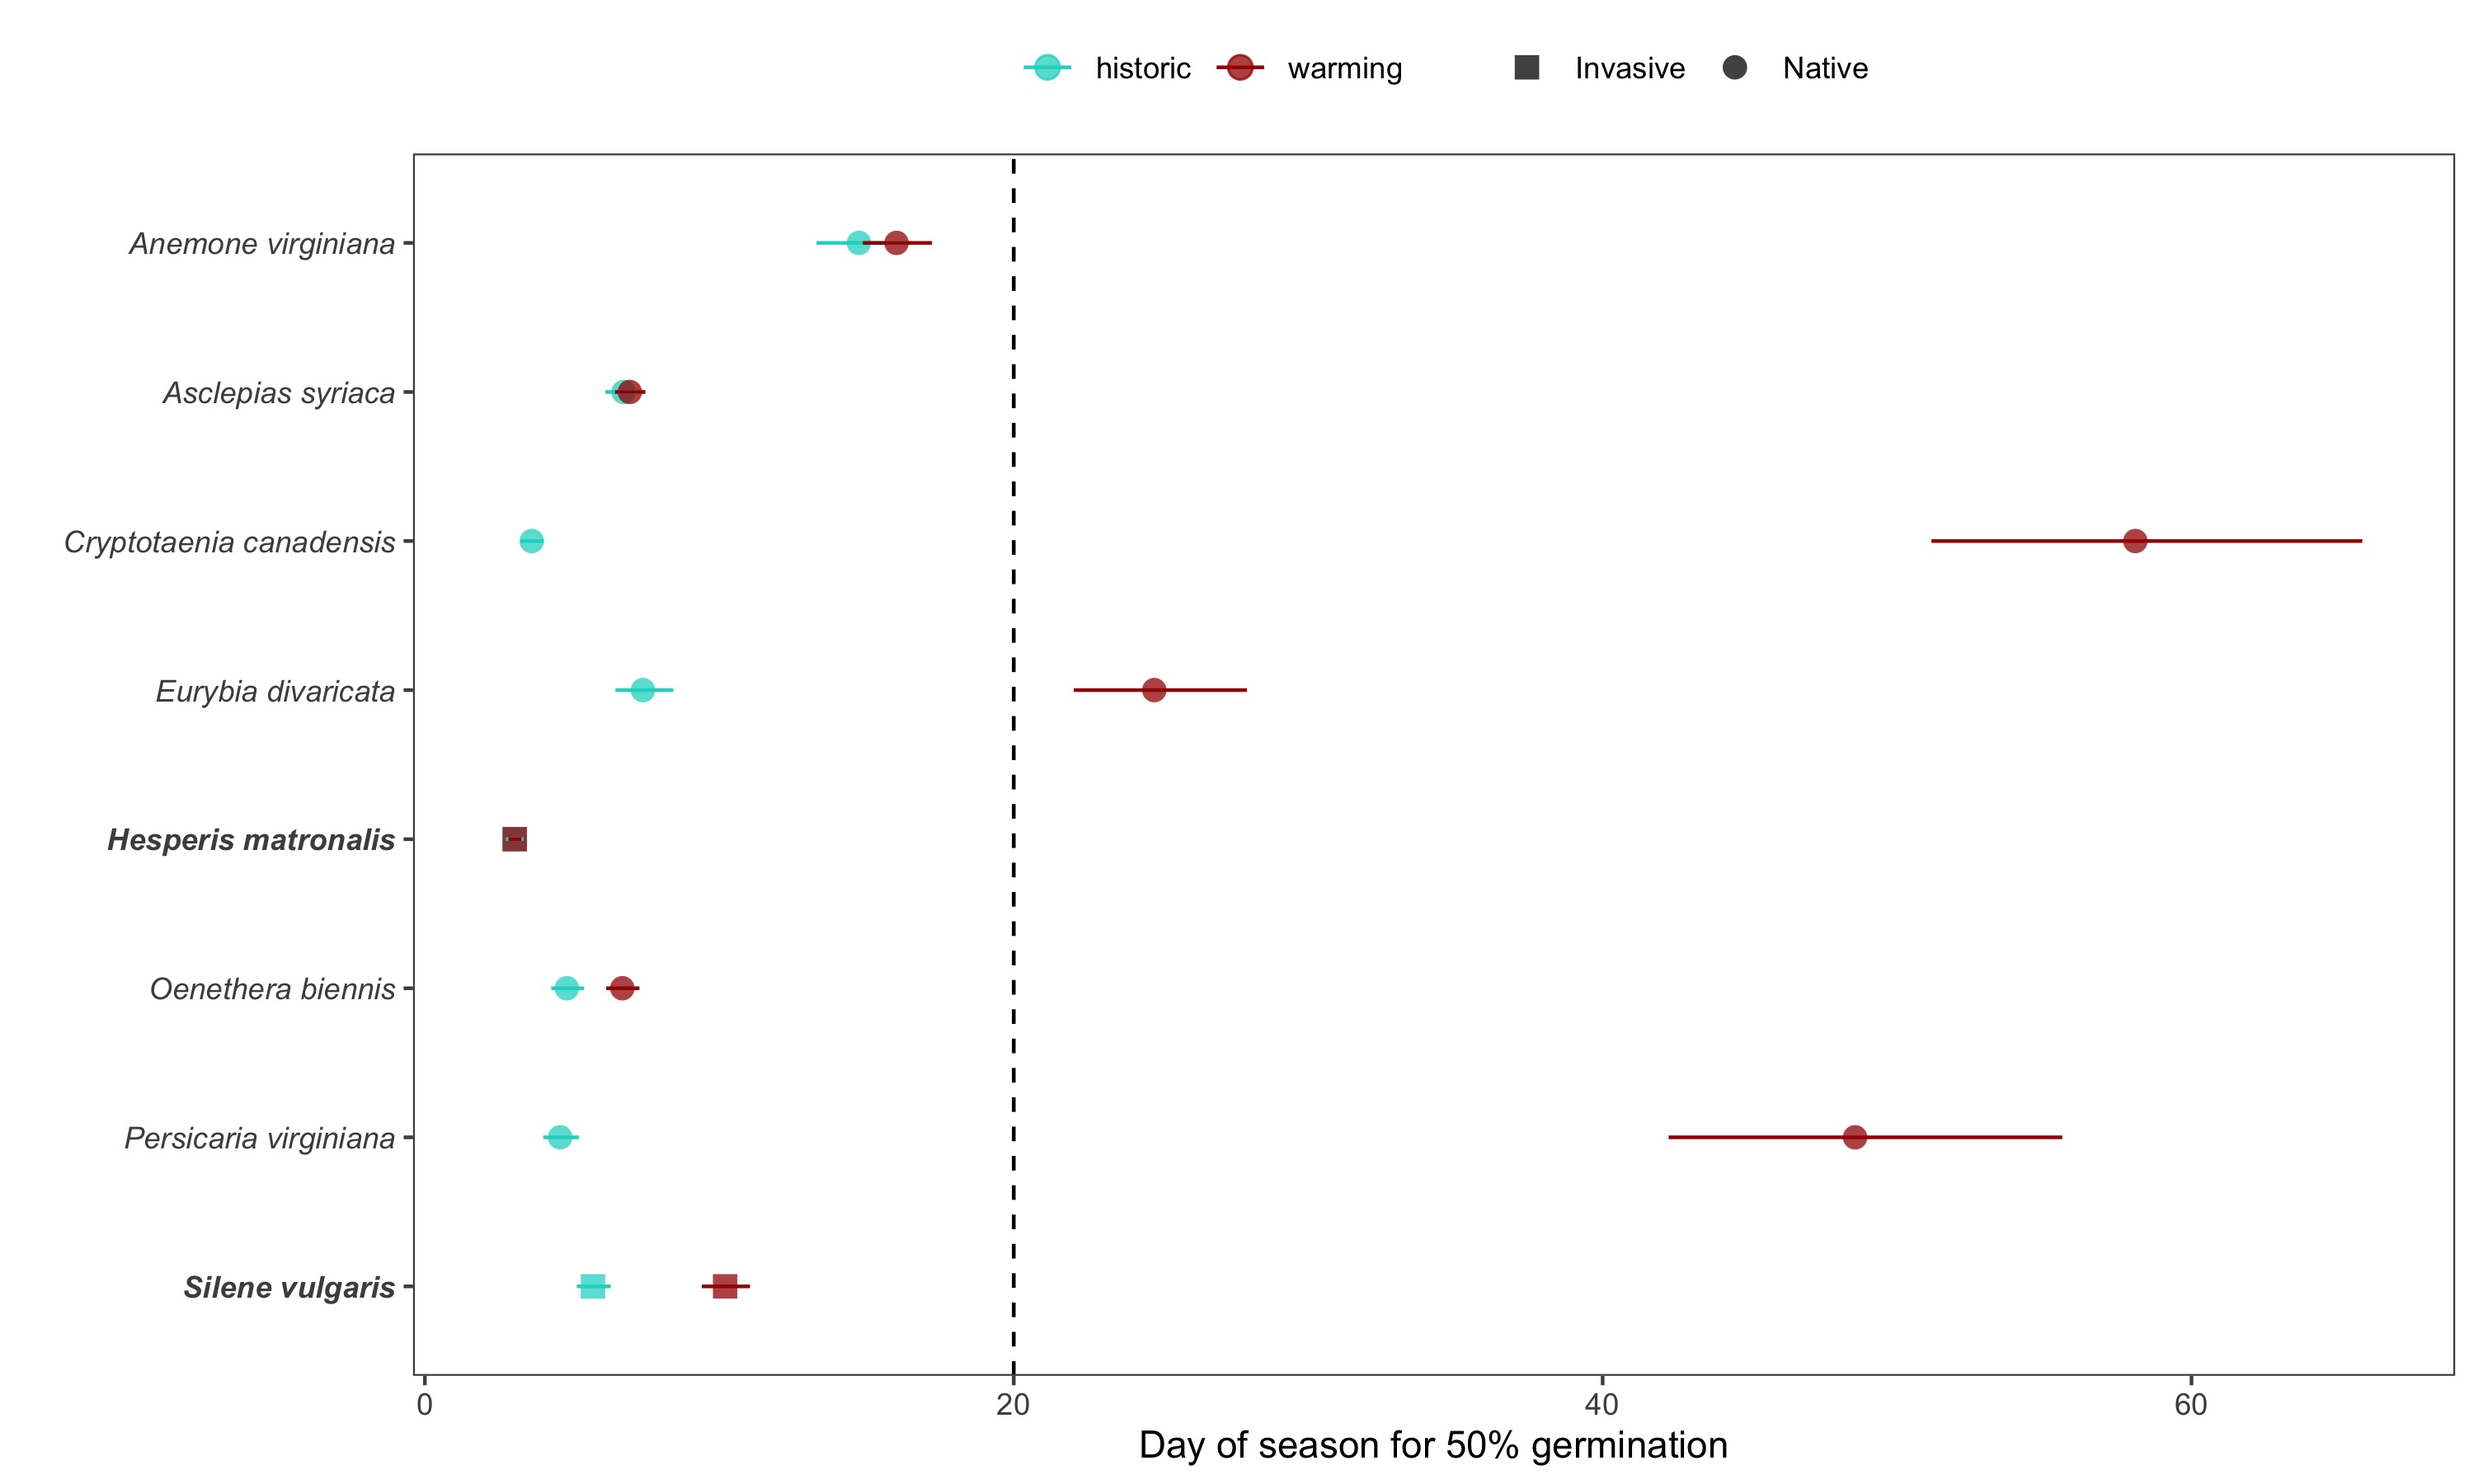
\includegraphics[width=\textwidth]{..//figure/commchange.jpeg}
   \caption{Predicted germination phenology of a suite of temperate herbs under varying cold stratification (6 vs. 10 weeks at 4\degree C) and incubation (20/10\degree C  vs. 25/15\degree C day/night) levels within the first 20 days of the growing period. Longer stratification periods increased the ratio of native to invasive species (cirlces vs. squares) that germinate within 20 days of the growing period, and reduced the phenological advantage of the invasive species in this study } 
   \label{fig:comm}
\end{figure}



%In combination our germination assays,The germination behavior of \texit{H. matronalis} was little affected by cold stratification, while germination rate and speed of \texit{C. canadensis} was strongly enhanced with cold stratification, especially when germianted at cooler temperatures (Fig. \ref{fig:aft}). These differences are themselves not surprising as \textit{H. matronalis} seeds are considered non-dormant \citep{}, and seeds of \textit{C. canadensis} are physiologically dormant \citep{}. , These different responses generated germination dynamics in which under alternative low stratification regimes \textit{H. matronalis} cohorts germinated as much as two weeks before \textit{C. canadensis}, while under high stratification, the species germinated at approximately the same time (Fig. \ref{fig:aft}). 

%In our competition trials, we observed that differences in germination on the order of a few days had substantial impacts on both the per capita and plot level relative growth rate differences among species (Fig \ref{fig:Cc},\ref{fig:RGRD}). If we consider the range of variability we observed (approximately two weeks lag to simultaneously)

%These inter-specific dynamics we observed are comparable to treatments applied in staggered planting experiments \citep{}, but the fact that we were able to induce these effects through varying the germination environment rather than directly manipulating germination itself is an important phase for translating the estimates from priority effect experiments into natural systems.  suggests that the kinds of seasonal priority effects may be important for realz, especially in seasonal environments with high levels of inte-rannual climate variations.



\end{document}

%\noindent We assessed the impact of competitor density and relative germination timing on species biomass with two different frameworks.

%First we calculated the average per-capita biomass of each species per pot, by divided each species' plot level biomass by its number of germinants. We then set up a system of pair-wise equations in which the per-capita biomass of each species was regressed against the density of con-specific seeds, density of competitor seeds, and the difference in mean germination time among them using Bayesian linear models. The equation is written below.
%
%\begin{align*}

%biomass_{C. canadensis}  &= \alpha +& \beta_{1}*density_{C. canadensis} + \beta_{2}*density_{H. matronalis}+\beta_{3}*$\delta$MGT + \epsilon} 

%biomass_{H. matronalis}  &= \alpha +& \beta_{1}*density_{C. canadensis} + \beta_{2}*density_{H. matronalis}+\beta_{3}*$\delta$MGT + \epsilon}

%\end{align*}

%
%In the formulation, the $beta$_1$ is the estimated effect of intra-specific competition, $beta_2$ is the estimated effect of inter-specific competition, and $beta_3$ is the estimated priority effect. From these estimates we calculated the competition coefficients (c) (ratio of intra- to inter-specific competition strength) for each species, with and without the additive effects of germination phenology differences.

%\begin{align*}
%
%$c_{sp1} $ &= $ \frac{b_{1}}{b_{2}} $

%$c_{prioritysp1}$ &= $\frac{(b_1+b_3)}{b_2}$

%\end{align*}
